\documentclass[12pt]{article}
%%% DOCUMENT FORMATTING %%%
\usepackage[margin=1in]{geometry}
\usepackage{enumitem}
\setlength{\parindent}{0pt}
\newcommand{\disp}{\displaystyle}

%%% HEADER %%%
\usepackage{fancyhdr}
\pagestyle{fancy}
\fancyhf{}
\lhead{MATH 1060}
\rhead{Vagnozzi}
\cfoot{\thepage}

%%% MATH NOTATION & SYMBOLS %%%
\usepackage{amssymb}
\usepackage{amsmath}
\newcommand{\R}{\mathbb{R}}
\newcommand{\N}{\mathbb{N}}
\newcommand{\Z}{\mathbb{Z}}
\newcommand{\lp}{\left(}
\newcommand{\rp}{\right)}
\newcommand{\ls}{\left[}
\newcommand{\rs}{\right]}
\newcommand{\lb}{\left\{}
\newcommand{\rb}{\right\}}
\newcommand{\arccot}{\text{arccot}}
\newcommand{\arccsc}{\text{arccsc}}
\newcommand{\arcsec}{\text{arcsec}} 

%%% TABLES %%%
\usepackage{colortbl}

%%% GRAPHS %%%
\usepackage{tikz}
\usepackage{pgfplots}
\pgfplotsset{compat=1.15}
\usepgfplotslibrary{fillbetween}
\usetikzlibrary{angles,quotes}

%%% ENVIRONMENTS %%%
\newcommand{\Example}{\paragraph{\Writinghand \hspace{0.1mm} Example.}}
\newcommand{\ExampleCont}{\paragraph{\Writinghand \hspace{0.1mm} Example (continued).}}
\newcommand{\boxenv}[2]{
	\fbox{
	\begin{minipage}{0.97\textwidth}
	\vspace{2mm}	
	\paragraph{#1} #2
	\vspace{2mm}
	\end{minipage}
	}}

%%% FUN THINGS %%%
\newcommand*\tc[1]{\tikz[baseline=(char.base)]{
            \node[shape=circle,draw,inner sep=2pt] (char) {#1};}}
\usepackage{marvosym}

%%% MISC %%%
\usepackage{hyperref}


\setcounter{page}{64}

\begin{document}
\section*{3.3: Differentiation Rules}

\boxenv{Learning Objectives.}{Upon successful completion of Section 3.3, you will be able to\dots
		
	\begin{itemize}[leftmargin=6mm]
		\item Answer conceptual questions involving rules of differentiation.
		\item Use graphs and tables to find derivatives.
		\item Find derivatives using rules of differentiation.
		\item Solve applications involving rules of differentiation.
		\item Simplify products and quotients to find their derivatives.
		\item Use derivatives to find slope locations and equations of tangent lines.
		\item Find higher order derivatives of functions.
		\item Use derivatives to evaluate limits.
		\item Use a calculator to approximate limits.
	\end{itemize}
	\vspace{-4mm}
}

\vspace{5mm}

\subsection*{Derivative Rules}

Now that we have a conceptual foundation for the derivative through our understanding of limits, it would be beneficial to speed up the process of finding derivatives without having to utilize the limit definition each time. We can find derivatives more efficiently using several \textbf{derivative rules}. In MATH 1060, you may use these derivative rules unless you are specifically asked to find a derivative \underline{by definition}.

\vspace{3mm}

\paragraph{Constant Functions.} The derivative of a \textbf{constant function}, i.e. a function $f(x)=c$ where $c\in R$, is

$$f'(x)=\lim_{h\to 0}\frac{f(x+h)-f(x)}{h}=\lim_{h\to 0}\frac{c-c}{h}=\lim_{h\to 0}0=0.$$

\vspace{3mm}

If we think of the derivative as the instantaneous rate of change, then this function must be zero because a constant function never changes.

\newpage

\paragraph{Linear Functions.} Consider $f(x)=mx+b$. Then the derivative of $f$ is

$$f'(x)=\lim_{h\to 0}\frac{m(x+h)+b-(mx+b)}{h}=\lim_{h\to 0}\frac{mh}{h}=\lim_{h\to 0}m=m.$$

\vspace{3mm}

Hence, the derivative of a \textbf{linear function} is its slope.

\vspace{40mm}

\paragraph{Power Functions.} Let $f(x)=x^n$ for $n\in\R$, i.e.\ the power is any real number. The derivative of $f$ is\dots 

\vspace{20mm}

This result is often referred to as the \textbf{power rule}. This rule simplifies derivatives immensely. To see how, consider the function $y=x^{1000}$. Finding the derivative of $y$ by definition would be extremely tedious.

$$y'=\lim_{h\to 0}\frac{(x+h)^{1000}-x^{1000}}{h}$$

\vspace{3mm}

Applying the power rule, we can see much more quickly that the derivative is\dots

\vspace{15mm}

\textit{Proof of the Power Rule.} Let $f\, :\, \R\rightarrow \R$ be defined as $f(x)=x^n$ where $n\in\N$ and suppose $f$ is differentiable at $x$. By the Binomial Theorem from algebra, we have

\begin{align*}
(x+h)^{n} &= {n \choose 0}x^{n}h^{0} + {n \choose 1}x^{n-1}h + {n \choose 2}x^{n-2}h^{2} + ... + {n \choose n-1}xh^{n-1} + {n \choose n}x^{0}h^{n}\\ &= x^{n} + nx^{n-1}h + {n \choose 2}x^{n-2}h^{2} + ... + {n \choose n-1}xh^{n-1} + h^{n}.
\end{align*}

Subtracting the $x^n$ term from both sides, we have the equality

$$(x+h)^{n} - x^{n} = nx^{n-1}h + {n \choose 2}x^{n-2}h^{2} + ... + {n \choose n-1}xh^{n-1} + h^{n}.$$

(continued on next page)

\newpage
Then, dividing by $h$ on both sides, we obtain

$$\frac{(x+h)^{n} - x^{n}}{h} = nx^{n-1} + {n \choose 2}x^{n-2}h + ... + {n \choose n-1}xh^{n-2} + h^{n-1}.$$

\vspace{3mm}

Lastly, taking the limit on both sides as $h\to 0$, we have the desired result:

$$ f'(x) = \lim_{h \to 0}\bigg(nx^{n-1} + {n \choose 2}x^{n-2}h + ... + {n \choose n-1}xh^{n-2} + h^{n-1}\bigg) = nx^{n-1}. $$
\begin{flushright}
$\square$
\end{flushright}


\vspace{5mm}

\subsection*{Properties of Differentiation}

Recall that limits are \textbf{linear} functions and that derivatives are, by definition, limits. As a result, we can say that differentiation is a \textbf{linear operator}. This means that, for all $s,t\in\R$,

$$\frac{d}{dx}\lp s f(x) \pm t g(x)\rp= s f'(x)\pm t g'(x).$$

\vspace{3mm}

Linearity means that the operator ``ignores'' numeric coefficients and that it can be applied to each term individually in a sum or difference.

\Example Find the derivative of each of the following functions.

\begin{enumerate}
	\item[\tc{1}] $f(x)=2x^2+3x$
	
	\vspace{20mm}
	
	\item[\tc{2}] $f(x)=x^5+x^4+x^3+x^2+x+1$
	
	\vspace{20mm}
	
	\item[\tc{3}] $f(x)=4x^4+3x^3+2x^2+x-1$
	
	\vspace{20mm}
\end{enumerate}

\newpage

\paragraph{Fractional Powers.} The power rule applies to negative and fractional exponents as well as positive ones.

$$\frac{d}{dx}\lp\sqrt[b]{x^a}\rp=\frac{d}{dx}\lp x^{\frac{a}{b}}\rp=\frac{a}{b}x^{\frac{a}{b}-1}=\frac{a}{b} x^{\frac{a}{b}-\frac{b}{b}}=\frac{a}{b}x^{\frac{a-b}{b}}$$

\vspace{5mm}

\Example We showed (by definition) that the derivative of $y=\sqrt{x}$ is $y'=\frac{1}{2\sqrt{x}}$. Show that we can obtain the same result using the power rule.

\vspace{20mm}

\Example Find the derivative of each of the following functions.

\begin{enumerate}
	\item[\tc{1}] $y=\disp\frac{1}{x}-\frac{1}{x^2}+\frac{2}{x^3}-\frac{3}{x^4}$
	
	\vspace{20mm}
	
	\item[\tc{2}] $y=\sqrt{x}+\sqrt[3]{x}+\sqrt[4]{x}+\sqrt[5]{x}$
	
	\vspace{20mm}
	
\end{enumerate}


\Example Evaluate the following expression.

\vspace{5mm}

\hspace{10mm}$\disp\frac{d}{dx}\lp 2\sqrt{x}+\frac{3}{2}\sqrt[3]{x^2}+\frac{5}{4} \sqrt[5]{x^4}\rp$

\vspace{50mm}

\Example Suppose that $f'(1)=\pi$ and $g'(1)=e$. Find $\lp 2f-3g\rp '(1)$.

\vspace{50mm}

Note that derivatives of products and quotients require special rules that we'll discuss in Section 3.4. For now, you should \textbf{simplify} products and quotients to apply the rules from this section.

\Example Evaluate the following expression.

\vspace{5mm}

\hspace{10mm}$\disp\frac{d}{dx}\lp\frac{x^3-3x^2-2x}{x^2}\rp$

\newpage

\paragraph{Horizontal Tangents.} A \textbf{horizontal tangent} occurs when the slope of the tangent line is zero --- in other words, when the \textit{derivative} is zero. To find the location of horizontal tangent(s), set $f'(x)=0$ and solve for $x$. Horizontal tangents are significant in applied settings, which we'll see in Chapter 4. For now, you only need to know how to locate them.

\Example Consider $f(t)=t^3-27t+5$.
\begin{itemize}
	\item[\tc{1}] Find the equation of the tangent line to $f$ at $t=0$.
	
	\vspace{30mm}
	
	\item[\tc{2}] Locate all horizontal tangents ($t$-values).
	
	\vspace{30mm}
	
\end{itemize}

\Example Use the graph below to evaluate the expression $\sqrt[3]{g'(2)-f'(2)}$.

\begin{center}
            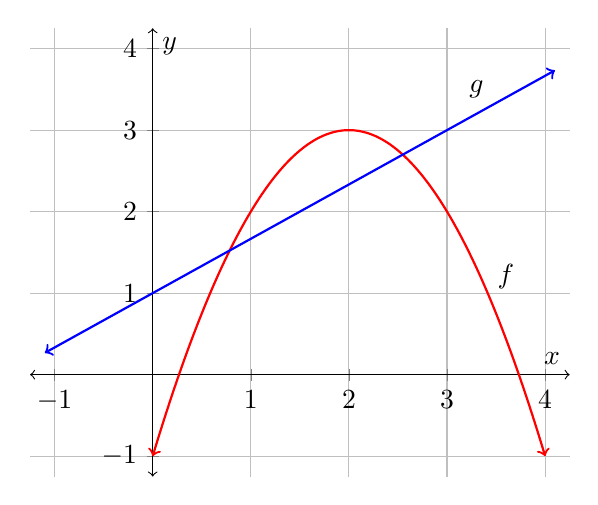
\begin{tikzpicture}
                \begin{axis}[
                	axis x line=middle,
			grid=both,
                	xmax=4.25, xmin=-1.25,
                	axis y line=center,
                	ymax=4.25, ymin=-1.25,
                	xlabel=$x$,ylabel=$y$,
                	axis line style=<->
%ticklabel style={inner sep=0.5pt,fill=white,opacity=1.0, text opacity=1}
                    ]
                    \addplot[name path=f,smooth,domain=0:4,color=red,samples=100,thick,<->] {-1*(x-2)^2+3};
                    \addplot[name path=f,smooth,domain=-1.1:4.1,color=blue,samples=100,thick,<->] {(2/3)*x+1};

		    \node at (3.3,3.5) {$g$};
		    \node at (3.6,1.2) {$f$};
                \end{axis}
            \end{tikzpicture}
        \end{center}
        
        \newpage
        
\paragraph{Exponential Functions.} The derivative of $f(x)=e^x$ is itself!

\vspace{20mm}

\boxenv{Remark.}{The slope of the exponential function $y=e^x$ at some point $x=c$ is simply $e^c$, which is the corresponding $y$-coordinate. The slope at $x=0$ is $e^0=1$.}

\vspace{5mm}

Be careful to avoid the common error of conflating the power rule and the exponential rule.

$$\frac{d}{dx}\lp e^x \rp\neq xe^{x-1}$$

\vspace{3mm}

Power functions have the variable in the \textit{base}, while exponential functions have the variable in the \textit{exponent}. 

\Example Find the derivative for each of the following functions.
\begin{itemize}
	\item[\tc{1}] $h(t)=\sqrt[4]{t}-4e^t+et^4$
	
	\vspace{20mm}
	
	\item[\tc{2}] $k(x)=e^x-x^e+ex+e$
	
	\vspace{20mm}
	
\end{itemize}

\paragraph{Higher-Order Derivatives.} If $f$ is a differentiable function, then $f'$ may also be differentiable. The derivative of $f'$ is called the \textbf{second derivative}.

$$f''(x)=\frac{d}{dx}\lp\frac{dy}{dx}\rp=\frac{d^2y}{dx^2}$$

\vspace{3mm}

We may also be able to continue taking the derivative to obtain \textbf{third derivatives} and beyond.

$$f'''(x)=f^{(3)}(x)=\frac{d}{dx}\lp\frac{d^2y}{dx^2}\rp=\frac{d^3y}{dx^3}$$

\vspace{3mm}

In general, the $n^\text{th}$ derivative may be denoted as follows.

$$f^{(n)}(x)=\frac{d^ny}{dx^n}$$

\newpage

\Example Find $f'$, $f''$, and $f'''$ for the following functions.

\begin{itemize}
	\item[\tc{1}] $f(x)=x^5-2x^3+10$
	
	\vspace{30mm}
	
	\item[\tc{2}] $f(x)=2e^x$
	
	\vspace{30mm}
\end{itemize}
\end{document}